% Deal with strides ?


\documentclass[a4paper]{article}
\usepackage[latin9]{inputenc}

\usepackage{a4wide}
\usepackage{alltt,url}
\usepackage{todonotes,graphicx}

% Because we have examples with project headers with accents in UTF8,
% restranlate them in latin9...
\usepackage{listingsutf8}
\lstset{inputencoding=utf8/latin9,language=C,
  numbers=left, numberfirstline=false, stepnumber=5, basicstyle=\small,
  keywordstyle=\bf}

% For various symbols:
\let\OldRightarrow=\Rightarrow
\RequirePackage{marvosym}
\let\MarvosymRightarrow=\Rightarrow
\let\Rightarrow=\OldRightarrow
\RequirePackage{wasysym}
% Deal with conflicts between ifsym and marvosym by renaming conflicting
% symbols:
\let\MarvosymLightning=\Lightning
\let\Lightning=\UnTrucIndefini
\let\MarvosymLetter=\Letter
\let\Letter=\UnTrucIndefini
\let\MarvosymSun=\Sun
\let\Sun=\UnTrucIndefini
\RequirePackage[weather,misc,alpine,clock]{ifsym}
\usepackage{amssymb}

\begin{document}

\title{Some implementation details from the \texttt{smecc} compiler}

\author{Ronan~\textsc{Keryell}~(\url{Ronan.Keryell@silkan.com})}

\maketitle

\tableofcontents{}


\section{Introduction}
\label{sec:introduction}

The shorter the better.

\section{OpenMP support}
\label{sec:openmp-support}

SME-C is a single program model (SPMD) based on OpenMP as its core model
with the OpenMP program being the controller of the whole application
driving some miscellaneous accelerators.

In our implementation, our compiler keep the OpenMP pragma in the output
main program.

The OpenMP pragma inside some piece of code mapped to accelerators may be
discarded if it does not make sense, for example if it is translated to an
OpenCL kernel or if it is replaced by a piece of hardware (FPGA...).


\section{Mapping on accelerators}
\label{sec:mapping-hardware}

The mapping of a function call on a specific piece of hardware can be
specified with pragma describing where the function is to be run and
optionally what arguments have to be transferred before execution and what
has to be retrieved after execution:
\begin{alltt}
#pragma smecy map(\emph{hardware[}, \emph{unit]*})
#pragma smecy arg(\emph{arg_id}, \emph{arg_clause[, arg_clause]...})
  some_function_call(...);
\end{alltt}

\begin{itemize}
\item \texttt{\emph{hardware}} is a symbol representing a hardware
  component of a given target such as \texttt{CPU}, \texttt{GPP},
  \texttt{GPU}, \texttt{PE}... They are target specific.
\item \texttt{\emph{unit}} entries are optional hierarchical instance
  number for a specific hardware part. This is typically an integer
  starting a 0. This hardware number can be an expression of the
  environment to be able to have a loop managing different accelerators.
\end{itemize}


\subsection{Mapping on OpenCL}
\label{sec:mapping-gpu}

The OpenCL can be used to target accelerators like GPU, STHORM or other
multicores.

For example the SME-C program

\lstinputlisting{examples/init_a.c}

is analyzed by the \texttt{smecc} compiler to generate an XML description
file to explain to the Par4All compiler that the \lstinline|init_array()|
function is parallel and has to be transformed to an OpenCL kernel, with
some memory transfers.

Then Par4All compiles the previous file to into 2 files, one for the host
program running on the main CPU:

\lstinputlisting{examples/init_a.p4a.c}

and an OpenCL file describing the kernel to be run on the accelerator:

\lstinputlisting{examples/p4a_wrapper_init_array.cl}

The OpenCL is indeed hidden in some higher-level macros beginning with
\verb|P4A_| to have terser code. For example
\verb|P4A_call_accel_kernel_2d| call the OpenCL API to compile the kernel,
stacking the call parameters and launching the kernel with the correct
NDRange. This allows to redirect more easily the compilation to CUDA for
example by changing the macro definitions.

Implementation limitations:
\begin{itemize}
\item an execution flow already mapped on a GPU kernel cannot launch
  another kernel because of the current OpenCL restriction\footnote{But
    this could be done in CUDA 5 with some recent K20 GPU.};
\item all the program has to be written in C, not C++.
\end{itemize}


\subsection{Mapping on STHORM MCA API}
\label{sec:prod-inform}

The STHORM platform is a MP-SoC with a 2-core ARM processor Cortex-A9
running Linux and an accelerator fabric with a 2D array of clusters, each
with 16 processing elements (PE).


\subsubsection{Addressing model}
\label{sec:addressing-model}

The MCA API contain the MCAPI message passing interface for embedded
system devices using an hierarchical addressing model made as a triplet
$<domain,node,port>$

\begin{figure}
  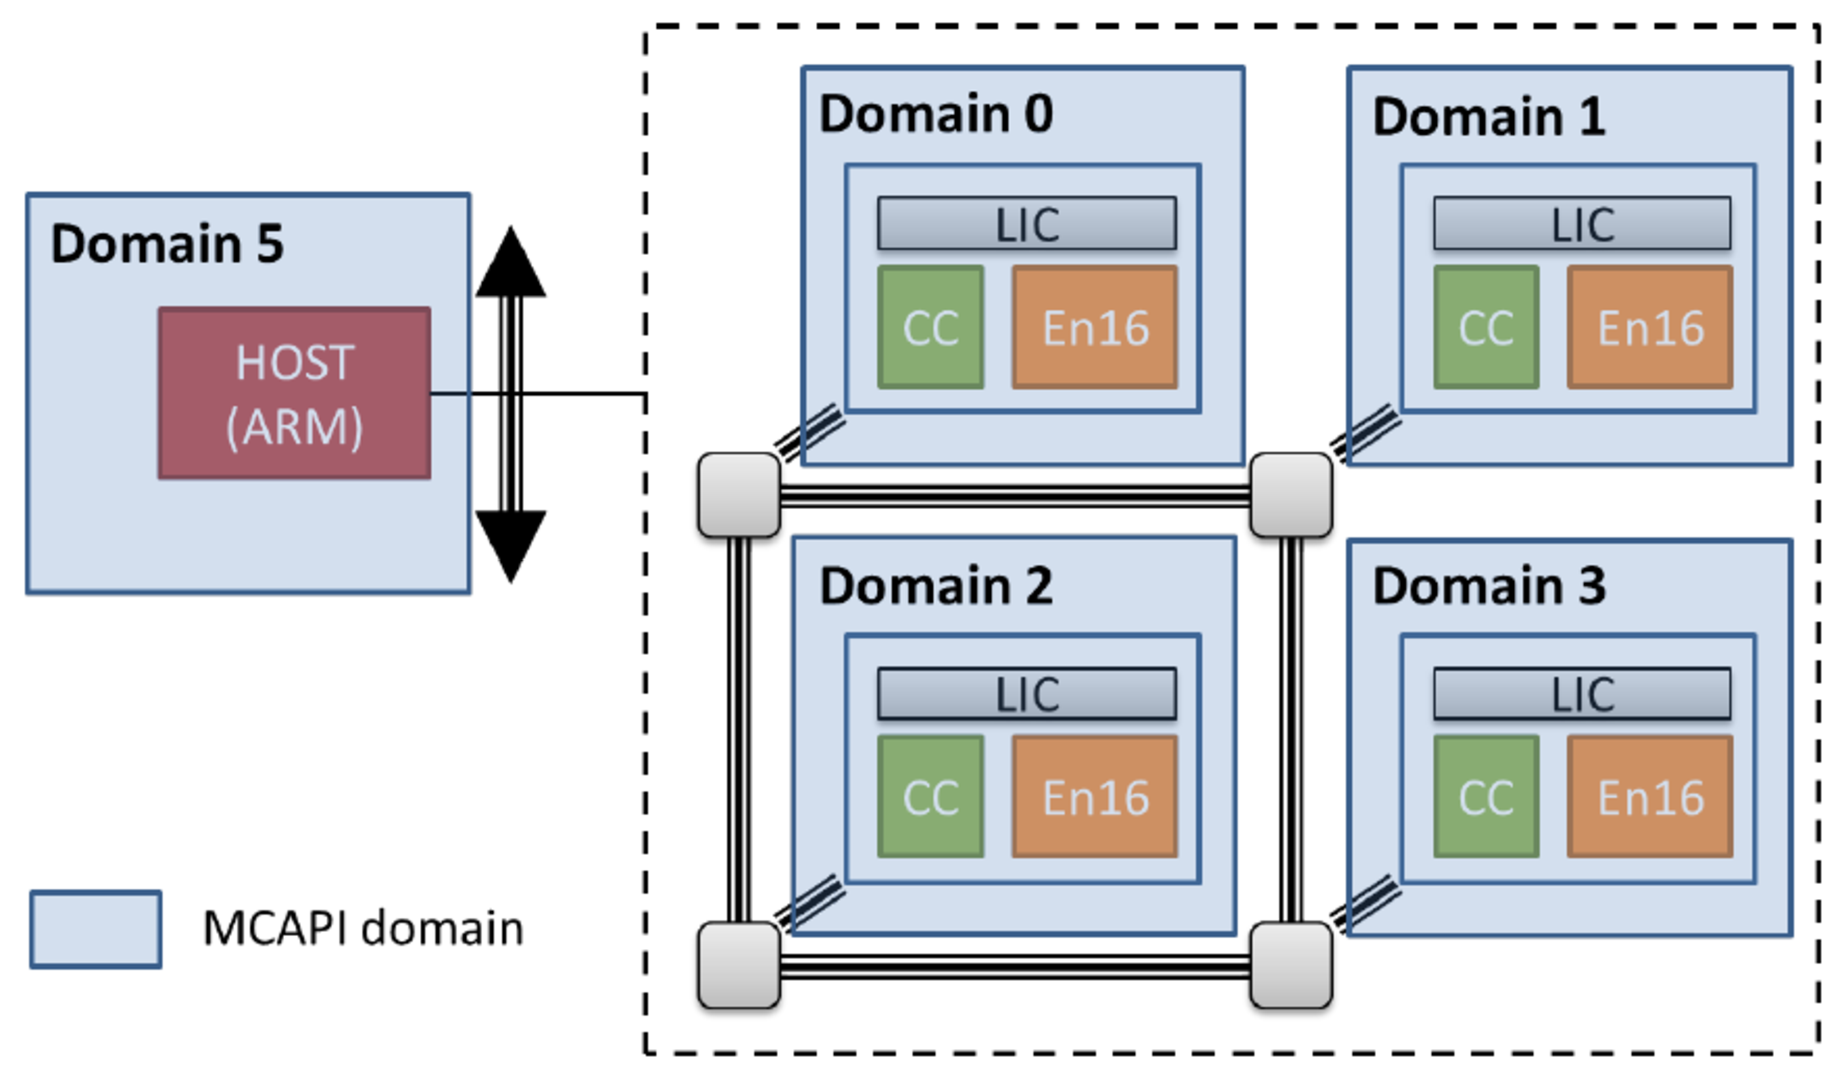
\includegraphics[width=\hsize]{figures/STHORM_MCAPI_mapping}
  \caption{MCAPI addressing model for a STHORM platform with $2\times2$
    clusters.}
  \label{fig:STHORM_MCAPI_mapping}
\end{figure}

The addressing model chosen by CEA for STHORM is to use the domain number
to select the clusters or the ARM host and use the node numbers to select
a PE inside the cluster selected by the domain number.

The domain numbering chosen by CEA for a cluster $(x,y)\in
(\mathbb{N}/n\mathbb{N})\times(\mathbb{N}/m\mathbb{N})$ inside a $n\times
m$ cluster machine is a plain 2D linearization:
\[
d = y \times n + x
\]
and the ARM host processor has the domain number $n\times m + 1$ with node
number 0.

An example for the $2\times2$ cluster simulator we use is shown on
Figure~\ref{fig:STHORM_MCAPI_mapping}.

Since the SME-C programming model is a SPMD model, by default all the code
runs on the host AMD processor, which is for example on domain 5 node 0,
perhaps with several OpenMP threads.

By using pragma such as
\begin{lstlisting}
#pragma smecy map(STHORM, 1, 3)
\end{lstlisting}
the execution of a function can be synchronously executed in the STHORM
fabric on the PE 3 of cluster 1.

Since for an execution on a PE the ARM processor has to launch a function
on it and there are many PEs, the function to be executed has to be large
grain.


\subsubsection{Memory model}
\label{sec:memory-model}

The memory model on STHORM is hierarchical and partially shared between
the ARM host processor and the fabric.

The global DDR memory, called the L3 memory, is shared in a weakly
coherent way by the host processor and the fabric PEs, through a global L2
cache.

This means that a multithread program running on the various cores and
with the right synchronization could run in parallel just by sharing
information though the L3 memory. Unfortunately, for power efficiency
reasons, there is no system like on a GPU to deal with coalescing multiple
accesses to the memory into a big one to improve
efficiency\todo{RK$\rightarrow$JM: does the L2 cache mitigates this?} of
the memory access. This means that the accesses will be slow.

To improve the efficiency, the local memory shared by the PEs of a cluster
or the private memory to a PE\todo{RK: double check it it makes sense.}
have to be used by placing the data in the right place.


\subsubsection{Runtime execution}
\label{sec:runtime-execution}

\todo{RK: express the following in some way with pragmas, comm}

Memory allocation

Our implementation is based on ST STHORM runtime. During nodes initialization and
channels connection we call ST memory allocators. User may want to use directly these memory
allocators. If it is the case user can refer to ST STHORM Runtime documentation [6]. Extract
of [6] which lists all the memory allocators accessible from CC :
\begin{lstlisting}
void * CC_l3Malloc (int size)
void CC_l3Free (void *ptr)
void * CC_enMalloc (int size)
void CC_enFree (void *ptr)
void * CC_malloc (int size)
void CC_free (void *ptr)
\end{lstlisting}


\section{Some design patterns for STHORM SME-C}
\label{sec:examples}

Here are some typical use-cases for the MCAPI STHORM target.

\todo{RK: no clear how to write an efficient application to use 64 PEs for
  example...}

\subsection{Same computation on all the PEs}
\label{sec:same-computation-all}

\lstinputlisting{examples/distribute_PEs.c}


\subsection{Same computation on all the PEs of a cluster}
\label{sec:same-computation-all-2}

\lstinputlisting{examples/independent_clusters.c}


\subsection{Stream computation through the PEs of a cluster}
\label{sec:stre-comp-thro}

\lstinputlisting{examples/stream_cluster_PEs.c}


\subsection{Systolic computation with the PEs of a cluster}
\label{sec:syst-comp-with}

\lstinputlisting{examples/systolic_PEs.c}


\subsection{Round robin computation on the clusters}
\label{sec:round-robin-comp}

\lstinputlisting{examples/round_robin_clusters.c}


%\lstinputlisting{examples/pipeline_cluster_PEs.c}

\end{document}


%%% Local Variables:
%%% mode: latex
%%% ispell-local-dictionary: "american"
%%% TeX-auto-untabify: t
%%% TeX-PDF-mode: t
%%% End:

% vim:spell spelllang=fr
